백트래킹(backtracking)은 해를 찾는 도중 해가 아니어서 막히면, 되돌아가서 다시 해를 찾아가는 알고리즘으로 최적화 문제와 결정 문제를 푸는데 쓰이며, 구현 시 재귀함수를 사용한다. 대표적인 문제들로 재귀함수의 사용법과 백트래킹을 익혀보자.

\section{이론}
스도쿠와 같은 퍼즐을 컴퓨터로 어떻게 풀 수 있을까? 가장 쉬운 방법은 모든 방법을 시도하는 것이다. 이를 위해 경우의 수를 셀 때 썼던 수형도(나뭇가지 그림)과 같은 아이디어를 쓸 수 있다. 첫 번째 칸에서 1~9 중 하나를 시도하고, 그 다음 칸에서 또 1~9중 하나를 시도하고, 이를 반복하는 완전 탐색을 하는 것이다. 빈 칸이 $t$개인 스도쿠를 푼다면, 총 $9^t$개의 경우를 시도하게 될 것이다.

하지만 꼭 모든 경우를 탐색해야 할까? 스도쿠에서 처음 두 칸에 모두 1을 채우는 것은, 뒤에 칸이 어떻게 채워지던지 불가능하다. 즉, 탐색을 하다가 중간에 불가능하다는 결론이 나오면 그 이후는 시도할 필요가 없다! 이 경우에는 다시 되돌아가서 다른 경우를 시도할 수 있다. 이처럼, 완전 탐색을 하되, 자명하게 불가능한 경우를 제외하여 시간의 효율을 조금 더 향상시킨 것이 백트래킹이다.

즉, 문제가 상수 개 중 하나를 선택하는 것을 여러 번 반복한다면, 백트래킹을 고려할 수 있다. 이때, 어느 순서로 채우는지에 따라 소요되는 시간이 크게 영향받을 수 있으므로, 좋은 방식을 찾는 것이 중요하다. 이제, 몇 가지의 예시 문제들로 백트래킹을 익히자.

\section{$N$-Queen 문제}
다음과 같은 문제를 생각해보자.
\begin{example}[$N$-Queen problem]\label{ex: n-queen}
    $N \times N$ 체스판 위에 $N$개의 퀸을 놓고자 한다. 가능한 경우가 존재하면 가능한 경우 한 가지를 출력하고, 그렇지 않으면 $-1$을 출력하라. 단, $N \leq 25$이다.
\end{example}
효율적 구현을 위해서는 어떤 순서로 선택을 할 지 결정해야 한다. 다음 관찰이 도움을 준다.

\begin{obs}
    한 가로줄에는 최대 하나의 퀸만 위치할 수 있다. 따라서 $N$개의 퀸을 놓으려면 정확히 하나의 가로줄에 하나의 퀸이 위치해야 한다.
\end{obs}

즉, 각 가로줄마다 하나의 퀸이 어디 위치할 지 $N$개 중에 하나를 선택하는 문제로 바꿀 수 있다. 이렇게 제일 위 가로줄부터 채우는 방식을 쓰기 위해 재귀함수 \texttt{solve}의 파라미터로 현재까지 퀸의 위치를 정한 가로줄의 개수 $L$을 사용할 것이다. 당연히 $L$은 현재까지 놓은 퀸의 개수와 같다. 그러면 \texttt{solve(L)}은 $L+1$번째 가로줄에 있는 $N$개의 칸에 퀸이 놓일 수 있는지 시험해 가능한 경우에 대해 모두 \texttt{solve(L+1)}을 호출하는 것으로 문제를 해결할 수 있다. 이 과정을 반복해 $L=N$에 도달하면 $N$개의 퀸을 놓았다는 뜻이므로, 현재 퀸의 위치를 출력하고 코드를 종료하면 된다. 만약 모든 경우를 시험했음에도 불구하고 코드가 종료되지 않았다면, 불가능하다는 뜻이므로 $-1$을 출력하고 코드를 종료하면 된다.

그렇다면 어떤 칸에 퀸이 놓일 수 있는지 어떻게 판단할 수 있을까? 그 퀸이 있는 세로줄, 가로줄, 그리고 두 방향에 대각선들에 있는 칸에 대해 다른 퀸이 있는지 확인하면 된다. 한 가로줄에 퀸 하나임은 보장되므로 가로줄은 확인할 필요가 없고, 아래쪽에 퀸이 없음이 보장되므로 위쪽에 있는 가로줄만 확인하면 된다. 이 과정은 정답 코드의 \texttt{isvaild(r, c)} 함수에서 처리된다.

\begin{code} \label{code: n-queen}
\Cref{ex: n-queen}의 정답 코드
\begin{lstlisting}
#include <bits/stdc++.h>
using namespace std;

int n, board[25][25];

bool isvaild(int r, int c) {
    for (int i = 0; i < r; i++) {
        if (board[i][c] == 1) return false;
    }

    int k = 1;
    while (true) {
        if (r + k >= n || c - k < 0) break;
        if (board[r + k][c - k] == 1) return false;
        k++;
    }
    k = 1;
    while (true) {
        if (r - k < 0 || c - k < 0) break;
        if (board[r - k][c - k] == 1) return false;
        k++;
    }

    return true;
}

void solve(int L) {
    if (L == n) {
        for (int i = 0; i < n; i++) {
            for (int j = 0; j < n; j++) cout << board[i][j] << " ";
            cout << "\n";
        }
        exit(0);
    }
    for (int i = 0; i < n; i++) {
        if (isvaild(L, i)) {
            board[L][i] = 1;
            solve(L + 1);
            board[L][i] = 0;
        }
    }
}

int main() {
    cin >> n;
    solve(0);
    cout << "-1\n";
    return 0;
}
\end{lstlisting}

\end{code}

\section{순열 구하기}

다음으로 백트래킹으로 주어진 조건을 만족하는 수열을 구하자. 고등학교 확률과 통계에서 배우는 것과 비슷한 느낌의 문제다.

\begin{example} $1 \leq M \leq N \leq 8$을 만족하는 두 정수 $N$과 $M$이 주어질 때, 각 조건을 만족하는 길이가 $M$인 \textbf{서로 다른 수열을 사전 순으로 모두} 출력하는 프로그램을 작성하라.
    \begin{itemize}
        \item (15649번) $1$부터 $N$까지 자연수 중에서 중복 없이 $M$개를 고른 수열
        \item (15650번) $1$부터 $N$까지 자연수 중에서 중복 없이 $M$개를 고른 \textbf{단조증가} 수열
        \item (15651번) $1$부터 $N$까지 자연수 중에서 \textbf{중복이 가능하게} $M$개를 고른 수열
        \item (15652번) $1$부터 $N$까지 자연수 중에서 \textbf{중복이 가능하게} $M$개를 고른 \textbf{단조증가} 수열
    \end{itemize}
\end{example}

이 문제에서도 \Cref{code: n-queen}에서 $L$에 대응하는 것을 잡아야 한다. 첫 번째 수부터 차례로 고르는 것이 제일 편하다. 따라서 현재까지 고른 수의 개수를 $L$로 두고 구현한다. 또한, 이 문제에서는 수열을 출력해야 하므로 지금까지 선택한 것을 저장해야 한다. 동적 자료구조인 \texttt{std::vector}을 아래와 같이 활용하면 편하다.

\begin{lstlisting}
#include <vector>
using namespace std;

vector<int> path;
void solve(int L) {
// ...
    path.push_back(i);
    solve(L+1);
    path.pop_back();
// ...
}
\end{lstlisting}

책에서는 이러한 방식을 재귀함수의 경로 기록이라고 할 것이다. 책에서 \texttt{path}라는 벡터 변수가 사용된다면, 함수 호출에 따른 경로를 기록한 경우가 많을 것이다.

이제 직접 네 문제를 구현해보라. 조건이 약간씩 다르기 때문에 세부적인 코드는 조금씩 변경해야 할 것이다. 이후의 과정은 독자에게 맡긴다.

이제, 비슷하지만 조금 더 어려운 문제를 보자.

\begin{example} $1 \leq M \leq N \leq 8$을 만족하는 두 정수 $N$과 $M$, 그리고 $N$개의 수로 이루어진 수열 $A_i$가 주어질 때, 각 조건을 만족하는 길이가 $M$인 \textbf{서로 다른 수열을 사전 순으로 모두} 출력하는 프로그램을 작성하라. 단, $N$개의 주어지는 수들 중에는 \textbf{같은 수가 있을 수 있다}.
    \begin{itemize}
        \item (15663번) 수열 $A_i$에서 중복 없이 $M$개를 고른 수열
        \item (15664번) 수열 $A_i$에서 중복 없이 $M$개를 고른 \textbf{단조증가} 수열
        \item (15665번) 수열 $A_i$에서 \textbf{중복이 가능하게} $M$개를 고른 수열
        \item (15666번) 수열 $A_i$에서 \textbf{중복이 가능하게} $M$개를 고른 \textbf{단조증가} 수열
    \end{itemize}
\end{example}

이 문제의 차이점은 $N$개의 수 중에 같은 수가 있을 수 있다는 것이다. 같은 수가 있으면, 이전 문제와 같은 방식으로 구현한 코드에서 출력하는 수열이 모두 다르다는 보장을 할 수 없다. 즉, 어떤 경우에 같아지는지 생각하고, 그 경우를 배제해야 한다. 같아지는 경우는 배열에 똑같은 수가 $a$번째와 $b$번째에 있을 때, 선택된 위치 중에서 $a$만을 $b$로 바꾼 경우이다. 즉, 아무것도 선택되지 않거나, $a$만 선택되거나, $a$와 $b$가 모두 선택되는 경우만 남기면 된다. 이것은 똑같은 수 중에서 더 앞에 있는 수가 선택되지 않았으면, 그 수를 선택하지 않는 방법으로 해결할 수 있다.

판단이 어렵다고 생각할 수 있지만, 배열을 처음에 정렬하고 시작함을 상기하자. 정렬된 배열에서 똑같은 수는 항상 연속된 위치에 있다. 이를 이용하면 구현을 쉽게 할 수 있다. 이후의 과정은 독자에게 맡긴다.

\section{격자 이동}
백트래킹을 사용하면 길을 찾을 수도 있다. 격자에서 상하좌우로만 이동할 수 있다면, 이것 자체도 4개 중에 하나를 선택하는 것을 반복하는 것이기 때문이다. 이와 관련된 문제를 하나 보자.

\begin{example} \label{ex: boj-1502}
    (1502번) $n \times m$ 격자에 두 개의 1이 적혀 있다. 두 개의 1 사이를 상하좌우로 인접한 칸으로 선을 그어 이으려고 한다. 선이 모든 칸을 다 지나야 할 때 가능한 이동 경로를 지나는 칸의 좌표로 출력하는 프로그램을 작성하라. 만약 가능한 경우가 없다면 \texttt{-1}을 출력한다. $m$과 $n$은 $2$ 이상 $8$ 이하의 짝수이다.
\end{example}

이 문제에서도 $L$에 대응하는 것을 생각하자. 지금까지 지난 칸의 수를 $L$로 잡으면 편하게 구현할 수 있을 것이다. 물론, 현재 칸에 따라 다음 칸이 달라지기 때문에 현재 칸의 위치를 나타내는 좌표도 파라미터로 넣어야 한다.

이 문제에 유용한 테크닉이 하나 있다. 격자에서 상하좌우로 이동하는 것은 현재 위치에서 $(-1, 0), (1, 0), (0, -1), (0, 1)$ 중 하나를 더하는 것과 같은데, 이것을 직접 작성해서 처리해도 되지만, 아래 코드와 같이 배열을 활용하면 조금 더 간단하게 할 수 있다.

\begin{lstlisting}
int dx[4] = {-1, 0, 1, 0}, dy[4] = {0, 1, 0, -1};

void solve(int L, int x, int y) {
// ...
    for (int k = 0; k < 4; k++) {
        int X = x + dx[k], Y = y + dy[k];
    }
// ...
}
\end{lstlisting}

이 방식은 상하좌우가 아니라 대각선까지 포함해 8칸이 이동 가능한 경우에도 비슷하게 적용할 수 있다. 이 방법을 사용하여 구현해보자. 만약, 구현 과정에서 시간 초과가 난다면 절대 불가능한 경우를 제외해 경우의 수를 줄여야 한다. 예를 들어 모든 칸을 지나지 않고 두 번째 1에 도착하는 경우는 절대 불가능한 경우이다.

\section{최적화}
이번에는 백트래킹에서 어떻게 불가능한 경우를 잘 추려내서 경우의 수를 줄일 수 있는지 예시를 통해 감을 익히자. 2048이라는 유명한 게임과 관련된 문제이다.

\begin{example}
    $N \times N$ 격자에서 2048 게임(\url{https://play2048.co/})을 시뮬레이션 하고자 한다. 실제 게임과 다르게 \textbf{블록의 생성이 없을 때}, 초기 상태에서 $X$번 이동하여 만들 수 있는 가장 큰 숫자를 구하는 프로그램을 작성하라.
    \begin{itemize}
        \item (12100번) $1 \leq N \leq 20$, $X = 5$
        \item (12094번*) $1 \leq N \leq 20$, $X = 10$
    \end{itemize}
\end{example}

$X=5$인 경우는 가능한 경우가 $4^5$으로 작기 때문에 완전 탐색을 해도 충분하다. 하지만, $X=10$인 경우, $N^2 \times 4^{10}$이 생각보다 커서 최적화가 필요하다. 일단 보드가 바뀌지 않는 경우 그 방향으로의 이동은 할 필요가 없다. 이는 자명한 최적화다.

정말 중요한 최적화는 문제에서 최댓값을 요구한다는 것이다. 즉, 현재 상황에서 어떻게 이동하더라도 최댓값이 갱신될 수 없으면 더 탐사할 필요가 없다. 이는 백트래킹 문제에서 자주 사용되는 중요한 테크닉이다. 더 구체적으로 말하면, 항상 최댓값은 많아야 2배 증가하므로, 현재 값에 남은 횟수 만큼 2를 곱한 값이 최댓값 이하라면 더 탐사할 필요가 없다.

상술한 두 가지 최적화를 추가하면 $X=10$인 경우에도 제한 시간 내에 문제를 해결할 수 있다.

\section{연습문제 A}
\begin{problem}
    \Cref{code: n-queen}의 시간 복잡도는 무엇인가?
\end{problem}
\begin{problem}
    \Cref{code: n-queen}에서 \texttt{isvaild(r, c)} 함수의 시간복잡도를 $T(n)$이라고 할 때 전체 시간복잡도를 $T(n)$으로 나타내라. 이 사실로부터 알 수 있는 것은 무엇인가?
\end{problem}
\begin{problem}
    $N=25$일 때, CPU의 연산 속도를 1초당 $10^{9}$회라고 가정하고 \Cref{code: n-queen}의 수행 시간을 구해보라. 예상되는 실행 시간은 얼마인가? 실제 실행 시간과 얼마나 차이나는가? 이 차이는 왜 발생하는가?
\end{problem}
\begin{problem}
    (9021번**) \Cref{ex: boj-1502}는 백트래킹을 사용하지 않고 수학적인 해법을 찾을 수 있다. 수학적인 해법을 찾아, $m$과 $n$이 $2$ 이상 $100$ 이하의 짝수인 경우를 해결해보라. 이렇게 각 문제마다 고유의 규칙을 찾아 답을 구성하는 것을 구성적(constructive)이라고 한다.
\end{problem}

\section{연습문제 B}

\begin{problem}
    (1128번) $N$개의 물건이 있고, 각 물건에는 무게와 가격이 있다. 또, 가방이 있는데, 가방에 담을 수 있는 무게의 최댓값은 $C$이다. 가방에 물건을 적절히 담아, 가방에 담긴 물건의 무게 합이 $C$ 이하이면서 가격의 합이 최대가 되도록 하려고 한다. 가능한 최댓값을 구하라. 단, $N \leq 50$, $C \leq 10^{16}$이고 물건의 무게와 가격은 모두 $10^{16}$ 이하이다. 또한, \textbf{물건의 무게는 모두 피보나치 수 중 하나이다}($1, 2, 3, 5, 8, 13, \cdots$).
\end{problem}

\begin{problem}
    (1799번) $N \times N$ 체스판에서 비숍을 놓을 수 있는 칸과 놓을 수 없는 칸이 주어질 때, 어떤 두 비숍도 공격당하지 않도록 놓을 수 있는 최대 개수를 출력하라. $N \leq 10$이다.
\end{problem}

\begin{problem}
    (5070번) 아래와 같은 모양의 퍼즐을 생각하자. 
    
    \begin{center}
        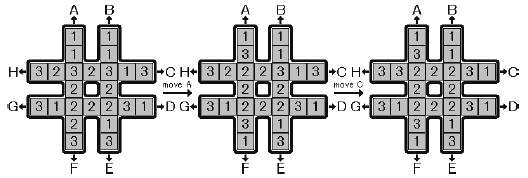
\includegraphics[width=0.5\textwidth]{Images/5070.png}
    \end{center}

    다음은 이 퍼즐에 대한 설명이다.
    \begin{itemize}
        \item 각 블록에는 1부터 3까지 수 중 하나가 적혀 있으며 각각은 정확히 8개씩 있다.
        \item 목표는 가운데 정사각형의 여덟 블록이 모두 같은 숫자가 되도록 하는 것이다.
        \item 사용할 수 있는 동작은 7개의 블록으로 이루어진 줄에서 끝 블록을 반대쪽 끝으로 이동시키고 나머지 여섯 개의 블록을 한 칸씩 미는 8가지의 동작이다. 각각의 동작은 A~H까지 라벨링되어 있다.
    \end{itemize}
    최소 횟수로 동작을 사용하여 퍼즐을 해결하려고 한다. 최소 횟수로 해결하는 방법들 중 사전순으로 가장 앞선 동작의 나열을 출력하고, 그 나열을 쓸 때 가운데 정사각형의 여덟 블록이 어떤 숫자가 되는지 출력하라.
\end{problem}

\begin{problem}
    (25795번) 화이트 초콜릿 조각과 다크 초콜릿 조각을 각각 $N$개를 붙여 초콜릿을 만들었다. 이 나열 중 특별한 조건을 만족하는 초콜릿을 예쁜 초콜릿이라고 한다.
    \begin{itemize}
        \item 화이트 + 다크 는 예쁜 초콜릿이다.
        \item 화이트 + 예쁜 초콜릿 + 다크 는 예쁜 초콜릿이다.
        \item 예쁜 초콜릿 + 예쁜 초콜릿 은 예쁜 초콜릿이다.
        \item 위 세 가지 규칙으로 만들어지지 않는 나머지 초콜릿은 예쁜 초콜릿이 아니다.
    \end{itemize}
    초콜릿의 점수는 정수 $a$에서 시작해 왼쪽부터 화이트 초콜릿 조각이 있으면 $b$를 더하고 다크 초콜릿 조각이 있으면 $c$를 곱하여 계산한 값을 $10^5$으로 나눈 나머지이다. $N, a, b, c$가 주어질 때 예쁜 초콜릿들 초콜릿의 점수가 가장 높을 때 최댓값을 구하여라. $N \leq 15$이고 $a, b, c$는 모두 $10^5$ 이하이다.
\end{problem}

\section{연습문제 C}

\begin{problem} 
    (2071번) $N \times N$의 검은 돌만 놓여 있는 바둑판의 집의 개수를 세려고 한다. 기존의 바둑과 다르게 모든 방향에서 블록으로 가려져 있는 곳만을 집으로 인정한다. 즉, 테두리는 둘러싸일 수 없으므로 집이 아니다. 하지만 바둑판을 이미 치워 바둑판의 모양은 알 수 없고 각 $N$개의 가로줄과 세로줄에 있는 바둑돌의 수, 각 $2N-1$개의 우상향과 우하향 방향의 대각선에 있는 바둑돌의 수만을 알고 있다. 이 정보를 입력으로 받아 바둑판에 있는 집의 크기를 계산하는 프로그램을 작성하라. 단, $N \leq 15$이고 주어진 정보로 바둑판의 모양을 유일하게 결정할 수 있음이 보장된다.
\end{problem}

\begin{problem}
    (2396번) 길이가 $L$인 막대 $M$개를 잘라 토막 $N$개를 얻었다. 다시 이 토막으로 길이가 같은 막대 여러 개를 만드려고 한다. 가능한 방법들 중에서 토막의 길이가 가장 짧을 때 그 길이를 출력하라. $N \leq 100$이고 토막의 길이도 $100$ 이하이다.
\end{problem}

\begin{problem}
    (18461번**) 길이가 $N$인 순열(permutation)에서 최장 증가 부분 수열(LIS)과 같은 길이를 가지며 교집합이 공집합인 증가하는 부분 수열 두 개가 존재하는 순열의 개수를 구하여라. $N \leq 75$이다.
    \begin{itemize}
        \item 길이가 $N$인 순열은 $1$부터 $N$까지의 수가 정확히 한 번씩 나타나는 수열이다.
        \item 증가 부분 수열은 길이 $N$의 주어진 수열에서 몇 개의 수를 제거하여 만든 증가 수열을 말하고, 최대 증가 부분 수열은 어떤 수열의 증가 부분 수열들 중 가장 긴 길이의 증가 부분 수열이다.
    \end{itemize}
\end{problem}

\begin{problem}
    (24258번*) $n$이 주어질 때 $a_1 a_2 a_3 \cdots a_n = a_1 + a_2 + \cdots + a_n$이며 $a_1 \geq a_2 \geq \cdots \geq a_n$인 순서쌍 $(a_1, a_2, \cdots, a_n)$의 개수를 출력하라. $2 \leq n \leq 10^{11}$이고 이러한 순서쌍의 개수는 주어진 조건에서 $10^{18}$개 미만임이 보장된다.
\end{problem}

\begin{problem}
    (26272번) $N$가지의 참-거짓 질문에 대한 대답 순서쌍이 모두 다른 $2^N$명의 사람들이 있다. 연구원은 매일 피실험자들을 대상으로 $2N$가지 유형의 실험을 진행하는데, $2i-1$번 유형의 실험에서는 $i$번 질문에 참이라 대답한 사람만 부르고, $2i$번 유형의 실험에서는 $i$번 질문에 거짓이라 대답한 사람만 부른다. 피실험자의 편의를 위해 연구원들은 이전 실험에 참가한 피실험자들 중 절반 이상이 다음 실험의 참여 대상이 되도록 순서를 정하려고 한다. 하지만 매번 실험 순서가 같다면 실험이 편향될 수 있기 때문에 연구자들은 $x$번 유형의 실험을 $y$번째로 시행할 수 있는 실험 시행 순서 중 가장 사전순으로 앞선 것을 택할 것이다. 여러분은 $Q$번 $x$와 $y$가 주어질 때마다 결정되는 실험 시행 순서 $a_k$를 구해 
    $$\sum_{k=1}^{2N} {ka_k}$$
    를 $10^9 + 7$로 나눈 나머지를 출력해야 한다. $2 \leq N \leq 10^9$이고, $1 \leq Q \leq 2\cdot10^5$이다.
\end{problem}

\newpage

\section{힌트}

\begin{hint}

\end{hint}

\begin{hint}

\end{hint}

\begin{hint}

\end{hint}

\begin{hint}
    thregium의 practice\_baekjoon 레포지토리
\end{hint}

\begin{hint}
    두 가지 최적화가 필요하다.
    \begin{itemize}
        \item 똑같은 무게를 가지는 여러 물건들 중에서 ?한 것을 먼저 골라야 한다.
        \item $C$ 이하인 가장 큰 피보나치 수부터 $t_1, t_2, \cdots$라 하면, 적당히 작은 상수 $k$에 대해 무게가 $t_1, t_2, \cdots, t_k$인 물건을 모두 고르지 않으면 [...]을 보장할 수 있다.
    \end{itemize}
\end{hint}

\begin{hint}
    N-Queen 문제와 비슷하게, 한 대각선에는 하나의 비숍만 놓일 수 있음을 활용해보자.
\end{hint}

\begin{hint}
    
\end{hint}

\begin{hint}
    모든 화이트 초콜릿을 자신보다 뒤에 있는 다크 초콜릿과 대응시키되, 모두 다른 다크 초콜릿과 대응시킬 수 있어야 예쁜 초콜릿이다. 이 조건은 현재까지 사용한 화이트 초콜릿의 개수와 다크 초콜릿의 개수로 쉽게 판별할 수 있다.
\end{hint}

\begin{hint}
    utilForever의 BOJ 레포지토리
\end{hint}

\begin{hint}
    hummingbird-12의 boj-solutions 레포지토리
\end{hint}

\begin{hint}
    \url{https://qoj.ac/contest/443}
\end{hint}

\begin{hint}
    총 다섯 개의 단계별 힌트가 있다.

    \textbf{[ 1 ]} \newline
    $i \geq j$인 $i$와 $j$에 대해 $(a_i, a_j)$에서 $(a_i+1, a_j-1)$로 바꾸면, 합은 일정하지만 곱은 감소한다. 즉, 합이 일정한 상황에서 곱의 최소는 $(a_1, 1, 1, \cdots, 1)$에서 갖는다. 그런데, $(a_1, 1, 1, \cdots, 1)$에서는 항상 합이 곱보다 크기 때문에, 실질적으로 $(a_1, 2, 1, \cdots, 1)$을 고려해야 한다. 이 상태에서 합보다 곱이 크다면 불가능하다. 이를 수식으로 풀면,
    $$2a_1 \leq n + a_1 \Rightarrow a_1 \leq n, a_1 \times a_2 \times \cdots \times a_n = a_1 + a_2 + \cdots + a_n \leq 2a_1 \leq 2n$$
    가 된다.

    \textbf{[ 2 ]} \newline
    이제, $a_2$부터 하나씩 결정하되, 곱으로 경우의 수를 줄일 것이기 때문에 $2$ 이상의 값으로 결정하자. 그러면 $2$ 이상의 값의 개수가 $2$개일 때부터($1$개는 불가능하다) $n$개일 때까지 모두 확인해야 하므로, 매번 아직 결정되지 않은 값을 모두 $1$로 두고 가능한 $a_1$이 존재하는지 판단하자. 재귀함수의 파라미터로는 $a_k$를 결정할 때의 $k$, $a_k$의 상한, 현재까지 합, 현재까지 곱을 넣으면 충분하다.

    \textbf{[ 3 ]} \newline
    \underline{곱에서 합을 뺀 값}을 점점 작아지게 만들어보자. 아래 부등식에서 각 순서쌍은, 곱에서 합을 뺀 값을 나타낸다.
    
    \begin{align*}
        (a_1, a_2, \cdots, a_n) \geq (a_1 + S, a_2, \cdots, a_k, 1, 1, \cdots, 1) \geq (a_1, a_2, \cdots, a_k, 1, 1, \cdots, 1) & \\ \textrm{where}~S = (a_{k+1}-1) + (a_{k+2}-1) + \cdots + (a_n-1) &
    \end{align*}

    즉, $a_k$까지 수를 정하고 그 이후는 $1$이라 가정한 뒤 가능한 $a_1$을 구했을 때, $a_2$보다 작으면 그 이후는 무조건 불가능하다. $(a_1=a_2, a_2, \cdots, a_k, 1, 1, \cdots, 1)$에서 곱에서 합을 뺀 값이 이미 양수이기 때문에, $(a_1 \geq a_2, a_2, \cdots, a_k, 1, 1, \cdots, 1)$에서도 양수이고, $(a_1, a_2, \cdots, a_k, a_{k+1}, \cdots, a_n)$에서도 양수가 되기 때문이다.

    \textbf{[ 4 ]} \newline
    \textbf{[ 3 ]}에 의해 $a_{k+1}$부터 전부 1일 때 가능한 유리수 $a_1$의 값이 $a_1$의 상한이 된다. 그리고 \textbf{[ 1 ]}에 의해 그 때 $a_1 + a_2 + \cdots + a_n$이 최대이다. 이렇게 구한 합의 상한과 하한 안에, $a_2 \times a_3 \times \cdots \times a_k$의 배수가 있어야 한다. 이를 활용하면 경우의 수를 더 줄일 수 있다.

    \textbf{[ 5 ]} \newline
    \textbf{[ 2 ]}를 확장해, $a_3$부터 하나씩 결정할 수 있다. 이 풀이의 장점은 현재까지의 곱에 따라 두 가지 방법을 사용할 수 있다는 것이다. $a_3 a_4 \cdots a_k$가 작을 때는 $a_2$의 상한이 $O \left( \sqrt{\frac{n}{a_3 a_4 \cdots a_k}} \right)$이므로, 가능한 $a_2$에 따라 $a_1$을 구한다. 반면, $a_3 a_4 \cdots a_k$가 클 때는 \textbf{[ 4 ]}와 같이 $a_1 + a_2 + \cdots a_n$의 값의 상한과 하한을 구하고, 그 범위에 속하는 $a_3 a_4 \cdots a_k$의 배수마다 이차방정식의 근의 공식으로 $a_1$과 $a_2$를 한번에 구하는 것이다. 이 방법은 $O(n \times (a_3 a_4 \cdots a_k)^{-2})$의 시간을 요구한다.
    
    \url{https://old.infosbg.com/Shumen_2021.html}
\end{hint}

\begin{hint}
    이 문제는 직접 규칙을 찾으며 주어진 입력에 따라 케이스를 나누어 수학적으로 해결할 수도 있다. 하지만, 여기서는 백트래킹 풀이에 대한 힌트를 수록한다.

    \textbf{[ 1 ]} \newline
    직전 점호 인원 중 절반이 넘게 소집해제되지 않는다는 것과, $a_k$와 $a_{k+1}$을 $2$로 나눈 몫이 다름은 동치이다.

    \textbf{[ 2 ]} \newline
    만약, $x$번 유형의 점호를 $y$번째로 실시해야 한다는 조건이 없다면, $1, 3, 2, 4, \cdots$와 같은 순서로 두는 것이 사전 순으로 가장 앞선다.

    \textbf{[ 3 ]} \newline
    \textbf{[ 2 ]}의 순서에서 $x$번 유형의 점호를 $y$번째로 실시하기 위해 원래 $x$번 유형이 있던 자리 주변과 $y$번째 주변의 순서를 바꾸어야 할 것이다. 각각에서 사전순 최소를 백트래킹으로 탐색하자.
\end{hint}